\documentclass[french]{article}
\usepackage[T1]{fontenc}
\usepackage{fullpage}
\usepackage{babel}
\usepackage{hyperref}
\usepackage{graphicx}
\usepackage[justification=centering]{caption}
\usepackage{amsmath}
\usepackage{amssymb}
\usepackage{listings}
\usepackage{xcolor}
\usepackage{parskip}

\lstset{
    inputencoding = utf8,  % Input encoding
    extendedchars = true,  % Extended ASCII
    literate      =        % Support additional characters
      {á}{{\'a}}1  {é}{{\'e}}1  {í}{{\'i}}1 {ó}{{\'o}}1  {ú}{{\'u}}1
      {Á}{{\'A}}1  {É}{{\'E}}1  {Í}{{\'I}}1 {Ó}{{\'O}}1  {Ú}{{\'U}}1
      {à}{{\`a}}1  {è}{{\`e}}1  {ì}{{\`i}}1 {ò}{{\`o}}1  {ù}{{\`u}}1
      {À}{{\`A}}1  {È}{{\`E}}1  {Ì}{{\`I}}1 {Ò}{{\`O}}1  {Ù}{{\`U}}1
      {ä}{{\"a}}1  {ë}{{\"e}}1  {ï}{{\"i}}1 {ö}{{\"o}}1  {ü}{{\"u}}1
      {Ä}{{\"A}}1  {Ë}{{\"E}}1  {Ï}{{\"I}}1 {Ö}{{\"O}}1  {Ü}{{\"U}}1
      {â}{{\^a}}1  {ê}{{\^e}}1  {î}{{\^i}}1 {ô}{{\^o}}1  {û}{{\^u}}1
      {Â}{{\^A}}1  {Ê}{{\^E}}1  {Î}{{\^I}}1 {Ô}{{\^O}}1  {Û}{{\^U}}1
      {œ}{{\oe}}1  {Œ}{{\OE}}1  {æ}{{\ae}}1 {Æ}{{\AE}}1  {ß}{{\ss}}1
      {ẞ}{{\SS}}1  {ç}{{\c{c}}}1 {Ç}{{\c{C}}}1 {ø}{{\o}}1  {Ø}{{\O}}1
      {å}{{\aa}}1  {Å}{{\AA}}1  {ã}{{\~a}}1  {õ}{{\~o}}1 {Ã}{{\~A}}1
      {Õ}{{\~O}}1  {ñ}{{\~n}}1  {Ñ}{{\~N}}1  {¿}{{?`}}1  {¡}{{!`}}1
      {°}{{\textdegree}}1 {º}{{\textordmasculine}}1 {ª}{{\textordfeminine}}1
      {£}{{\pounds}}1  {©}{{\copyright}}1  {®}{{\textregistered}}1
      {«}{{\guillemotleft}}1  {»}{{\guillemotright}}1  {Ð}{{\DH}}1  {ð}{{\dh}}1
      {Ý}{{\'Y}}1    {ý}{{\'y}}1    {Þ}{{\TH}}1    {þ}{{\th}}1    {Ă}{{\u{A}}}1
      {ă}{{\u{a}}}1  {Ą}{{\k{A}}}1  {ą}{{\k{a}}}1  {Ć}{{\'C}}1    {ć}{{\'c}}1
      {Č}{{\v{C}}}1  {č}{{\v{c}}}1  {Ď}{{\v{D}}}1  {ď}{{\v{d}}}1  {Đ}{{\DJ}}1
      {đ}{{\dj}}1    {Ė}{{\.{E}}}1  {ė}{{\.{e}}}1  {Ę}{{\k{E}}}1  {ę}{{\k{e}}}1
      {Ě}{{\v{E}}}1  {ě}{{\v{e}}}1  {Ğ}{{\u{G}}}1  {ğ}{{\u{g}}}1  {Ĩ}{{\~I}}1
      {ĩ}{{\~\i}}1   {Į}{{\k{I}}}1  {į}{{\k{i}}}1  {İ}{{\.{I}}}1  {ı}{{\i}}1
      {Ĺ}{{\'L}}1    {ĺ}{{\'l}}1    {Ľ}{{\v{L}}}1  {ľ}{{\v{l}}}1  {Ł}{{\L{}}}1
      {ł}{{\l{}}}1   {Ń}{{\'N}}1    {ń}{{\'n}}1    {Ň}{{\v{N}}}1  {ň}{{\v{n}}}1
      {Ő}{{\H{O}}}1  {ő}{{\H{o}}}1  {Ŕ}{{\'{R}}}1  {ŕ}{{\'{r}}}1  {Ř}{{\v{R}}}1
      {ř}{{\v{r}}}1  {Ś}{{\'S}}1    {ś}{{\'s}}1    {Ş}{{\c{S}}}1  {ş}{{\c{s}}}1
      {Š}{{\v{S}}}1  {š}{{\v{s}}}1  {Ť}{{\v{T}}}1  {ť}{{\v{t}}}1  {Ũ}{{\~U}}1
      {ũ}{{\~u}}1    {Ū}{{\={U}}}1  {ū}{{\={u}}}1  {Ů}{{\r{U}}}1  {ů}{{\r{u}}}1
      {Ű}{{\H{U}}}1  {ű}{{\H{u}}}1  {Ų}{{\k{U}}}1  {ų}{{\k{u}}}1  {Ź}{{\'Z}}1
      {ź}{{\'z}}1    {Ż}{{\.Z}}1    {ż}{{\.z}}1    {Ž}{{\v{Z}}}1
      % ¿ and ¡ are not correctly displayed if inconsolata font is used
      % together with the lstlisting environment. Consider typing code in
      % external files and using \lstinputlisting to display them instead.      
  }



\definecolor{codegreen}{rgb}{0,0.6,0}
\definecolor{codegray}{rgb}{0.5,0.5,0.5}
\definecolor{codepurple}{rgb}{0.58,0,0.82}
\definecolor{backcolour}{rgb}{0.95,0.95,0.92}

\lstdefinestyle{mystyle}{
    backgroundcolor=\color{backcolour},   
    commentstyle=\color{codegreen},
    keywordstyle=\color{magenta},
    numberstyle=\tiny\color{codegray},
    stringstyle=\color{codepurple},
    basicstyle=\ttfamily\footnotesize,
    breakatwhitespace=false,         
    breaklines=true,                 
    captionpos=b,                    
    keepspaces=true,                 
    numbers=left,                    
    numbersep=5pt,                  
    showspaces=false,                
    showstringspaces=false,
    showtabs=false,                  
    tabsize=2
}

\lstset{style=mystyle}
\setlength{\parindent}{0pt}

\hypersetup{
  colorlinks=true,
  linkcolor=black,
  urlcolor=blue
}

\graphicspath{ {./img/} }
\title{%
    \huge Adrenaline.AI  \\
    \bigskip
    \large E4 - Mise en situation \\ 
    Développeur en Intelligence Artificielle,
    titre professionnel enregistré au RNCP - École IA Microsoft by Simplon
    \vfill
    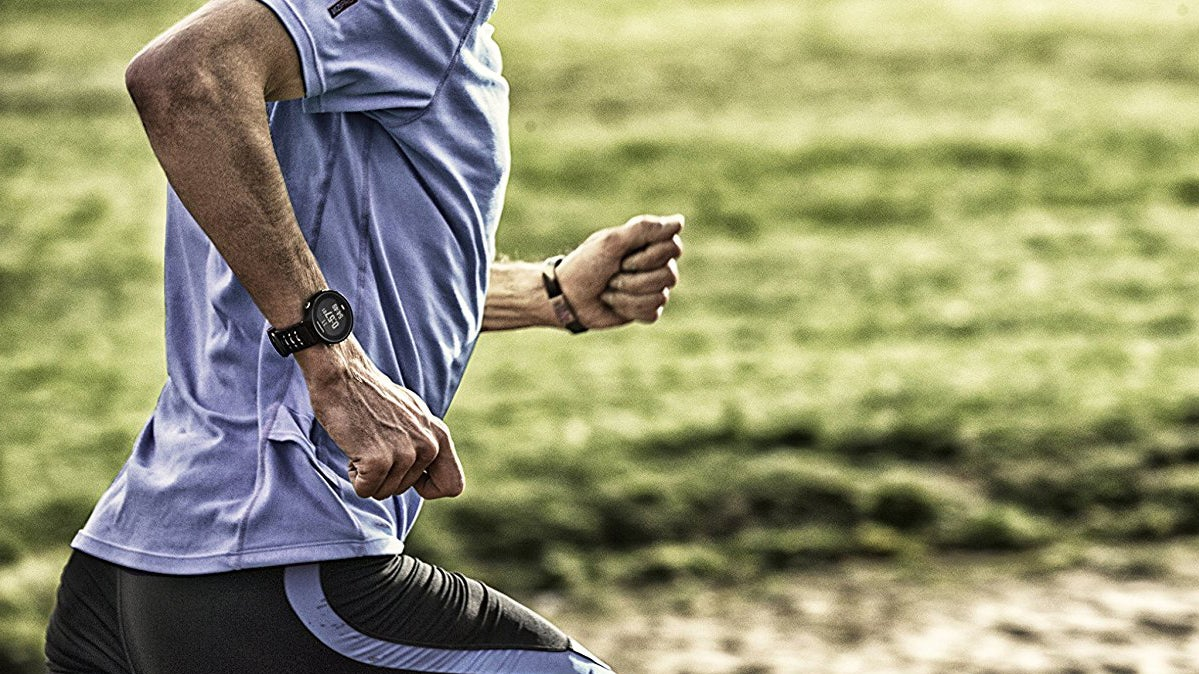
\includegraphics[width=14cm]{running.jpeg}
    \vfill}
\date{29 mars 2024}
\author{par Vincent Papelard}

\begin{document}
    \renewcommand{\contentsname}{Table des Matières}
    \renewcommand{\refname}{Références}
    \maketitle
    \pagenumbering{arabic}
    \pagenumbering{gobble}
    \newpage
    \tableofcontents
    \newpage
    \pagenumbering{arabic}

    \section*{Introduction}

    Nous sommes contactés par un fabricant d'équipements de sport et de montres connectées. Cette entreprise propose, entre autres, un site internet où sont publiés des programmes de course à pied génériques que les sportifs peuvent suivre pour s'améliorer. Cependant, elle aimerait bien passer à la vitesse supérieure en proposant des entraînements personnalisés selon la forme physique et l'expérience sportive des coureurs. Toutes ces données sont déjà disponibles grâce au modèle de montre connectée qu'elle commercialise et qui remporte un franc succès. Les data scientists de notre client travaillent déjà sur ce projet qu'ils ont baptisé \textbf{Adrenaline.AI}, mais ils n'ont personne dans leur équipe pour créer l'interface qui donnera accès à cette fonctionnalité. Notre rôle est donc de concevoir, développer et déployer la preuve de concept d'une application qui permettra aux utilisateurs de voir les entraînements personnalisés qui leur sont proposés.
    
    Le code de ce projet est disponible sur GitHub (\href{https://github.com/vinpap/adrenaline.ai}{https://github.com/vinpap/adrenaline.ai}). L'application et la base de données sont déployées sur \textbf{Microsoft Azure} (l'application est disponible sur \href{https://vincent-adrenaline-ai.azurewebsites.net/}{https://vincent-adrenaline-ai.azurewebsites.net/}).
    \section{Cahier des charges}

    Afin de formaliser au mieux le processus de développement et de s'assurer que l'application créée répond bien aux attentes du client, un cahier des charges est établi en discutant avec lui.

    \subsection{Objectifs}

    Quatre objectifs d'Adrenaline.AI ont été identifiés :
    \begin{itemize}
        \item \textbf{Objectif 1} : permettre à l'utilisateur de consulter en toute autonomie un entraînement de course à pied quotidien généré selon les données physiques captées par sa montre connectée (rythme cardiaque, temps de sommeil, calories brûlées et distance parcourue chaque jour en kilomètres)
        \item \textbf{Objectif 2} : encourager l'utilisateur à faire confiance aux recommandations d'entraînement en justifiant le choix des séances proposées
        \item \textbf{Objectif 3} : permettre à l'utilisateur de visualiser la progression quotidienne de plusieurs indicateurs clés : rythme cardiaque moyen au repos, calories brûlées, temps de sommeil et distance parcourue
        \item \textbf{Objectif 4} : sécuriser l'accès aux données des utilisateurs pour que seuls ces derniers puissent voir les informations les concernant.
    \end{itemize}

    \subsection{Description fonctionnelle des besoins}

    Voici les fonctionnalités attendues par le client pour remplir ces objectifs. Chacune d'entre elles remplit un ou plusieurs objectifs, indiqués entre parenthèses.
    \begin{itemize}
        \item \textbf{Fonctionnalité 1} (répond aux objectifs 1 et 2) : l'application contient une page web qui affiche le contenu détaillé de la recommandation d'entraînement du jour. On notera que l'application peut également conseiller au coureur de se reposer aujourd'hui si elle juge que c'est nécessaire (après une mauvaise nuit de sommeil, par exemple). Le descriptif de la séance d'entraînement est accompagné d'un court texte qui explique le choix de cet entraînement. Voici quelques exemples de justifications possibles :
        \begin{itemize}
            \item pour une séance d'endurance fondamentale (course lente) : "cette séance vous permet d'améliorer votre forme physique générale afin de vous préparer à des entraînements plus dificiles"
            \item pour une séance de fractionné (alternance de périodes de course rapide et de récupération) : "cette séance vous aide à maintenir une vitesse soutenue pendant de longues sorties"
            \item pour un jour de repos (pas de course à pied) : "pas de course à pied aujourd'hui afin de récupérer après la séance difficile d'hier"
        \end{itemize}
        \item \textbf{Fonctionnalité 2} (répond à l'objectif 3) : l'application contient une page web qui permet de visualiser la progression de plusieurs valeurs clés mesurées par la montre du coureur :
        \begin{itemize}
            \item le rythme cardiaque moyen au repos
            \item le temps de sommeil
            \item le nombre de calories brûlées
            \item la distance parcourue en kilomètres
        \end{itemize}
        Ces valeurs sont exprimées de manière quotidienne (e.g. nombre de kilomètres parcourus un jour donné).
        \item \textbf{Fonctionnalité 3} (répond aux objectifs 1, 2, 3) : l'application tire ses données d'une base de données relationnelle. Cette base de données contient les informations de tous les utilisateurs de montres connectées. Ces données sont uploadées depuis les téléphones portables des utilisateurs lorsqu'ils synchronisent leur montre et leur téléphone en Bluetooth.
        \item \textbf{Fonctionnalité 4} (répond à l'objectif 4) : les utilisateurs doivent s'authentifier via une page dédiée pour pouvoir utiliser l'application. Des mécanismes de sécurité sont mis en place pour empêcher quelqu'un d'accéder de façon non autorisée aux données des utilisateurs.
    \end{itemize}
    \subsection{Livrables attendus}
    Dans le cadre de ce projet, les éléments suivants doivent être livrés au client :
    \begin{itemize}
        \item une instance opérationnelle de l'application sur un serveur 
        \item la base de données nécessaire au fonctionnement de l'application, hébergée sur un serveur distinct de l'application
        \item une documentation qui explique comment installer l'application et ses dépendances
        \item le code source du projet, sur une plateforme en ligne (e.g. GitHub ou GitLab).
    \end{itemize}
    \subsection{Ressources et délais}

    Notre client dispose de moyens limités et ne souhaite pas payer et gérer lui-même un serveur dédié pour y déployer l'application et la base de données. À la place, il souhaite ne payer que pour les ressources de calcul réellement nécessaires à l'application. Il veut également réduire le travail nécessaire en termes de maintenance pour ne pas avoir à payer une équipe dédiée à cette tâche.
    
    Le projet doit être finalisé et les livrables présentés ci-dessus transmis au client avant le \textbf{31 mai 2024}.
    \section{Outils et environnement technique}

    Suite à l'établissement du cahier des charges, il est nécessaire de choisir les bons outils et méthodes de travail pour garantir le respect des demandes du client.
    \subsection{Environnement de production}

    Dans le but de répondre au mieux au désir du client de réduire les coûts de déploiement et de maintenance, la plateforme de cloud \href{https://azure.microsoft.com/fr-fr/}{Azure} de Microsoft a été choisie pour héberger l'application et la base de données. Azure offre plusieurs avantages qui rendent cette solution particulièrement adaptée aux besoins de ce projet :
    \begin{itemize}
        \item Azure offre de nombreux tarifs différents pour l'hébergement d'application et de bases de données. Dans le cas où les ressources allouées au projet seraient insuffisantes ou excessives, le client peut ajuster son tarif via le portail d'Azure pour optimiser ses coûts
        \item les serveurs physiques sont gérés par Azure, ce qui limite la maintenance à réaliser du côté de notre client
        \item Azure propose de nombreux services, y compris des services d'hébergement de modèles d'intelligence artificielle. Les data scientists d'Adrenaline.AI pourront donc déployer leur IA sur Azure s'ils le souhaitent.
    \end{itemize}

    Ces avantages rendent aussi Azure intéressant sur le plan de \textbf{l'éco-responsabilité}. En effet, installer des serveurs directement chez notre client poserait un problème d'efficacité energétique puisque ces serveurs fonctionneraient continuellement, et ce quel que soit le traffic auquel ils sont soumis. Une partie de la puissance de calcul de ces serveurs serait donc "perdue" durant les périodes où les serveurs reçoivent peu de requêtes. En comparaison, les fournisseurs de cloud comme Azure couvrent avec de grands centres de données les besoins en calcul de nombreux clients. Cette mise en commun des besoins de multiples clients leur permet donc de facilement activer ou désactiver des ressources de calcul en fonction des besoins, ce qui mène à une diminution de la consommation d'énergie au total.

    En ce qui concerne les outils et langages de développement, nous utiliserons :
    \begin{itemize}
        \item \textbf{Python}, et plus spécifiquement le framework \textbf{Flask}, pour coder le serveur de l'application web.
        \item \textbf{HTML}, \textbf{CSS} et \textbf{JavaScript} pour coder l'interface de l'application
        \item \textbf{MySQL} pour implémenter la base de données.
    \end{itemize}
    \subsection{Gestion de projet}
    \begin{figure}[h!]
        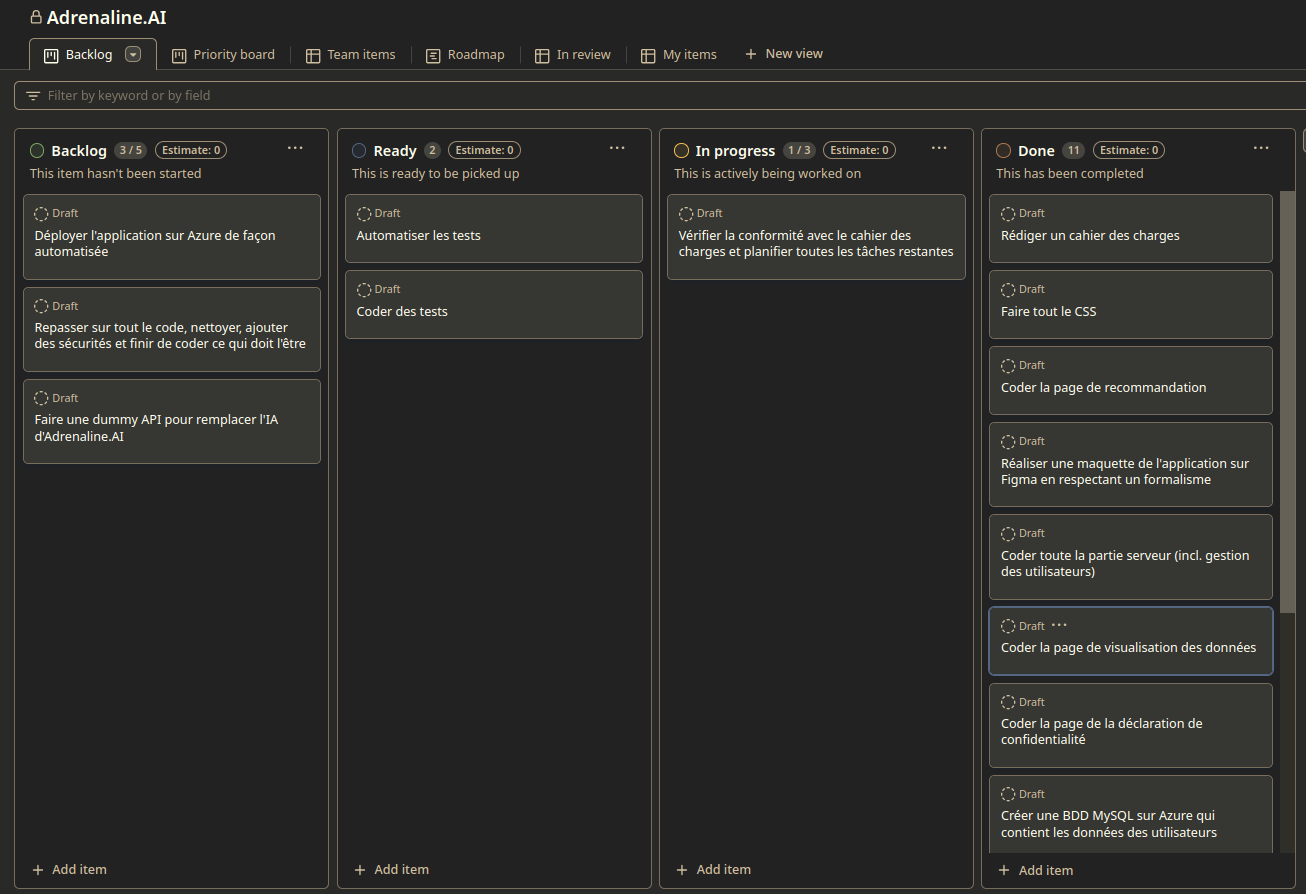
\includegraphics[width=12cm]{kanban}
        \centering
        \caption{Tableau kanban du projet. On remarque que des limites sont imposées au nombre de tâches non commencées ou en cours.}
        \centering
    \end{figure}

    La réalisation de ce projet a été planifiée sur une période de quatre semaines à raison de deux jours complets de travail par semaine. Cela équivaut à environ 56 heures de travail au total.

    Le travail nécessaire à ce projet a été organisé en utilisant la méthode \textbf{kanban}. Cette technique de gestion de projet repose sur l'utilisation d'un tableau qui recense les différentes tâches avec leur statut (terminées, à revoir, en cours, etc...). Un aspect important de ce tableau est qu'il limite le nombre de tâches présentes dans chaque colonne. L'objectif est de limiter la charge de travail sur les personnes qui travaillent sur le projet et de les encourager à terminer leurs tâches (plutôt que de disperser leurs efforts sur un grand nombre de tâches). Dans le cadre de ce projet, le tableau Kanban proposé par GitHub a été utilisé.

    Pour compléter l'utilisation de ce tableau, un \textbf{bilan des tâches en cours} a été réalisé tous les jours passés sur ce projet, en début de journée. Ce bilan d'une dizaine de minutes environ vise à faire le point sur les tâches en cours et à venir pour s'assurer que celles-ci sont toujours pertinentes. Il arrive en effet que des tâches initialement planifiées se révèlent finalement non nécessaires ou superflues. Faire un point en début de journée permet donc de commencer à travailler avec une vision claire des tâches de la journée tout en s'assurant de leur pertinence.

    \section{Conception de l'application}

    Cette section détaille l'étape de conception qui a été réalisée dans le cadre du développement d'Adrenaline.ai. La conception de ce projet consiste en l'élaboration de deux éléments :
    \begin{itemize}
        \item un \textbf{diagramme de flux de données} qui explicite les différents processus et entités nécessaires au fonctionnement du projet et détaille la circulation des informations entre eux
        \item une \textbf{maquette} qui présente les différentes pages web de notre application ainsi que les interactions qui les lient.
    \end{itemize}
    \subsection{Diagramme de flux de données}
    Le diagramme de flux de données présenté sur la page suivante expose les différents processus nécessaires au fonctionnement de l'application. Il comporte quatre types d'éléments :
    \begin{itemize}
        \item les \textbf{entités} : il s'agit des personnes et composants externes à l'application qui communiquent avec celle-ci. Dans notre cas, il existe deux entités : l'utilisateur qui interagit avec l'application, et le modèle d'intelligence artificielle qui est sollicité par l'application pour générer un entraînement recommandé en fonction des données d'un utilisateur
        \item les \textbf{processus} : on peut les assimiler à des fonctions qui travaillent avec les données qu'elles reçoivent et communiquent avec des entités, ou d'autres processus
        \item les \textbf{sources de données} : ce sont les fichiers, bases de données ou autres supports d'information qui stockent les données utilisées par les différents processus
        \item les \textbf{flux de données}, représentés par des flèches : ils modélisent les transferts de données entre les différents processus, entités et sources de données.
    \end{itemize}
    Ce diagramme expose principalement trois grands processus : l'inscription d'un nouvel utilisateur, la connexion d'un utilisateur existant et la génération d'un entraînement personnalisé pour un utilisateur. On notera que le modèle d'intelligence artificielle est ici présenté comme une entité externe à l'application. En effet, on part ici du principe que ce modèle sera disponible via un composant externe tel qu'une API et ne fait donc pas partie de l'application à proprement parler.

    \newpage
    \begin{figure}[h!]
        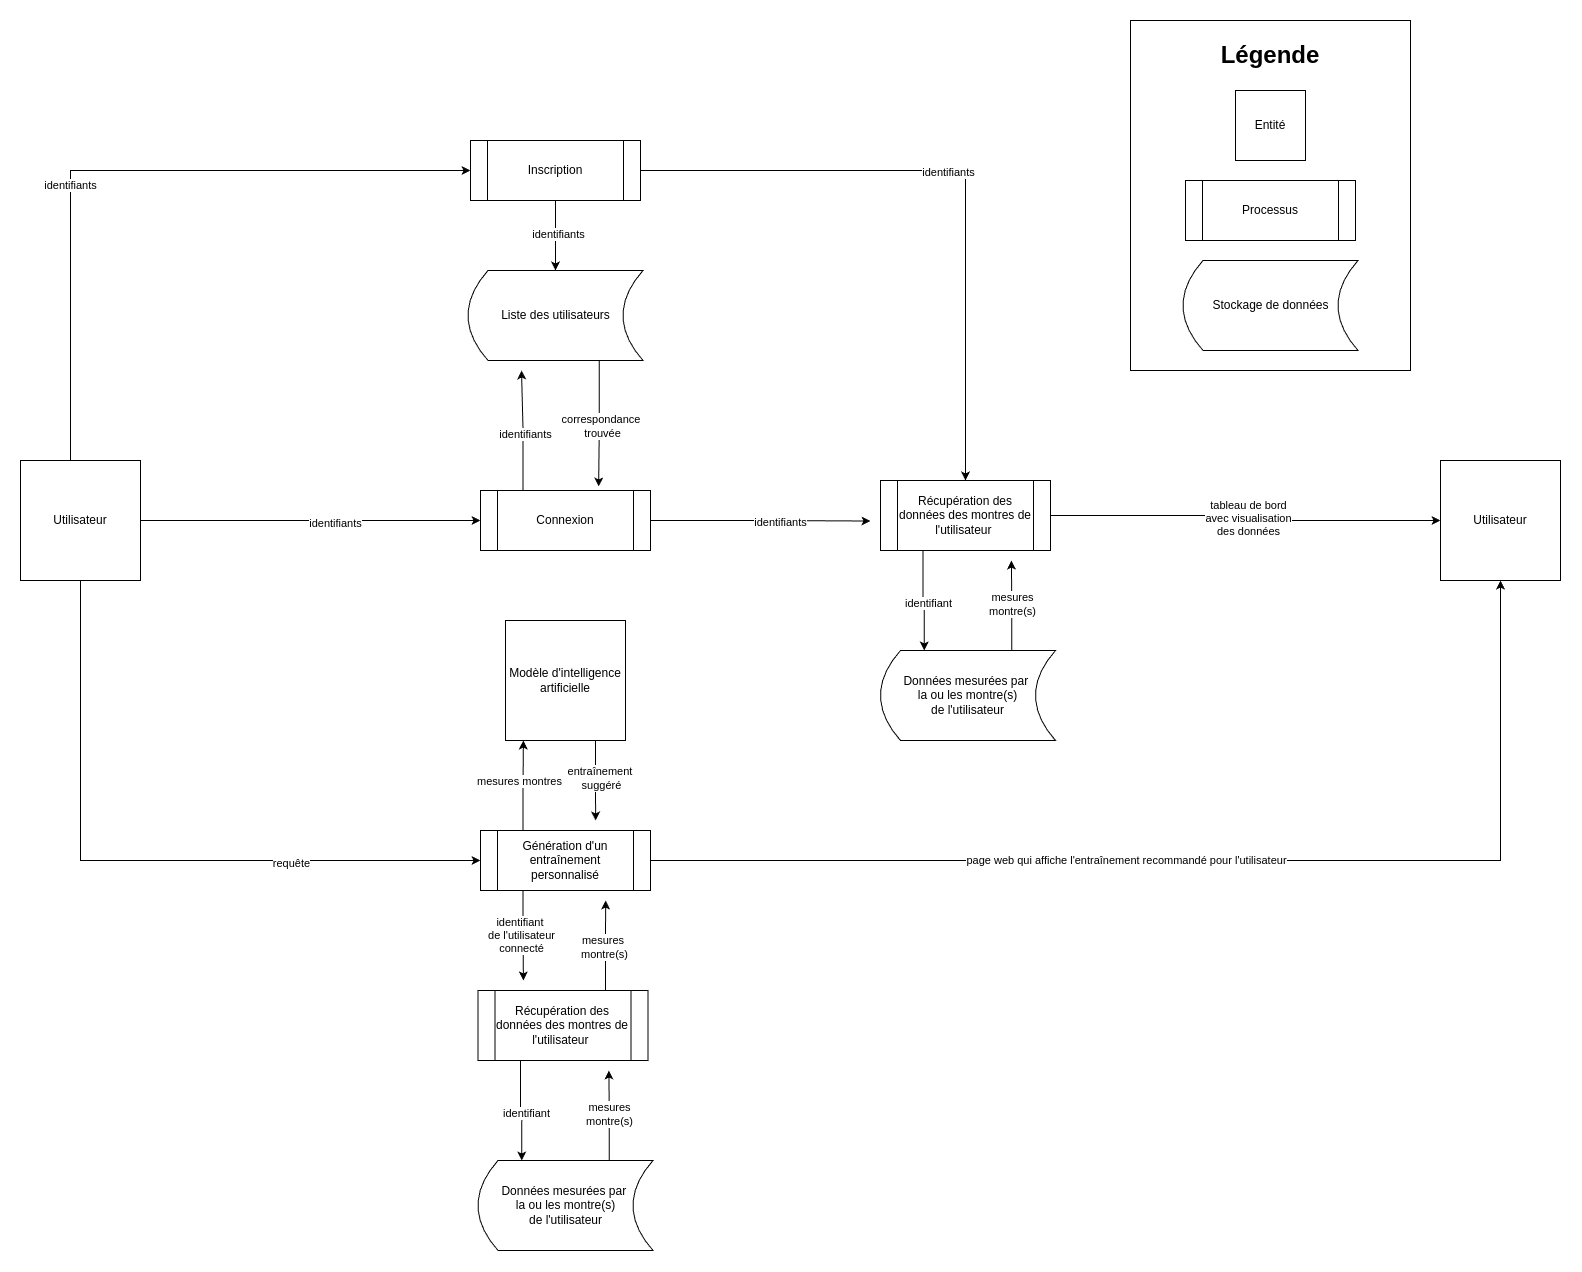
\includegraphics[width=15cm]{dataflow_e4}
        \centering
        \caption{Diagramme de flux de données qui représente le fonctionnement de l'application. Il modèlise trois grands processus de l'application : l'inscription d'un nouvel utilisateur, la connexion d'un utilisateur existant et la génération d'un entraînement personnalisé pour un utilisateur}
        \centering
    \end{figure}
    \subsection{Maquette}
    Le diagramme de flux de données nous a donné un aperçu du fonctionnement général de l'application. La prochaine étape de ce projet est la conception d'une maquette pour représenter l'interface de notre future application web. Ceci nous permettra d'avoir un support visuel qui nous permet d'identifier les pages web à coder et nous serivra de modèle général lors de l'implémentation du front-end. 
    
    Cette maquette est réalisée à l'aide de \href{https://www.figma.com/}{Figma}, un outil de conception graphique en ligne. La maquette est disponible sur la plateforme via \href{https://www.figma.com/design/bnhI3kF6nxTpzE3eWSHdCg/Adrenaline.AI?m=dev&node-id=3-15&t=JgaLgxLw4a6ylK5V-1}{ce lien}.
    \begin{figure}[h!]
        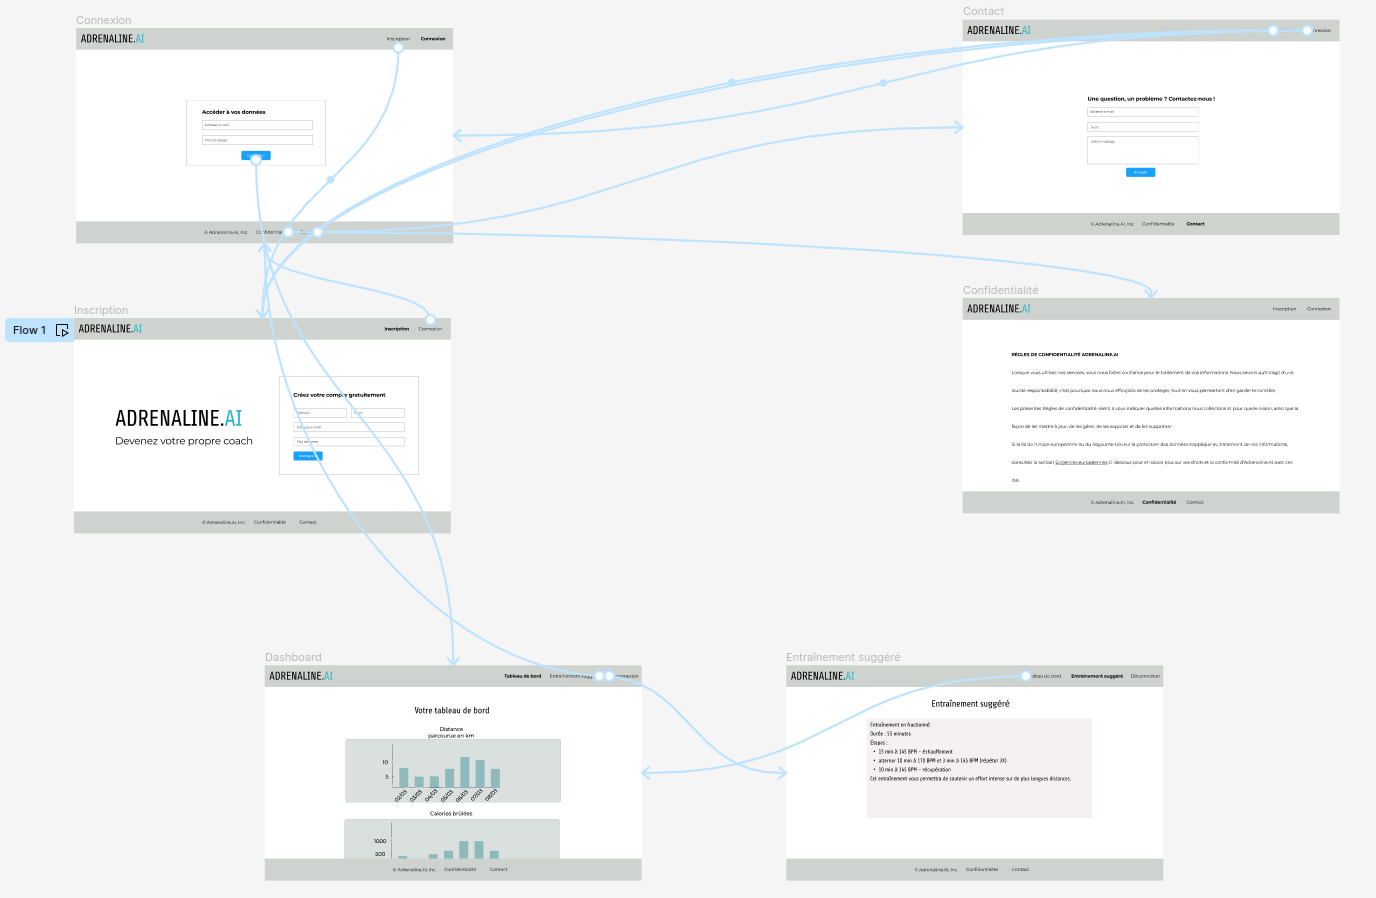
\includegraphics[width=12cm]{figma}
        \centering
        \caption{Vue d'ensemble de la maquette réalisée sous Figma. Les flèches bleues qui relient les pages web entre elles représentent un parcours possible de l'utilisateur sur l'application, autrement dit l'un des cheminements qu'il peut suivre en cliquant sur les diférents éléments de l'interface. Figma offre la possibilité de naviguer soi-même sur la maquette comme si on était sur une vraie application. Cela permet de vérifier que notre design est ergonomique pour l'utilisateur.}
        \centering
    \end{figure}

    Cette étape de maquettage est importante pour concevoir une interface claire et ergonomique où l'utilisateur arrive rapidement à la page qu'il cherche. Les fonctionnalités de prototypage de Figma nous permettent de naviguer nous-mêmes sur la maquette de notre application, ce qui est utile pour détecter les éventuels problèmes d'ergonomie.
    La maquette de notre application comporte six pages qui assurent les fonctionnalités suivantes :
    \begin{itemize}
        \item \textbf{Connexion} : permet de se connecter via un formulaire. C'est la page d'accueil par défaut pour les utilisateurs qui ne sont pas déjà authentifiés
        \item \textbf{Tableau de bord} : cette page montre les dernières mesures envoyées par l'utilisateur sous forme de graphiques. Accéder à la page d'accueil du site en étant authentifié redirige vers cette page
        \item \textbf{Inscription} : permet de créer un compte via un formulaire d'inscription
        \item \textbf{Entraînement suggéré} : présente à l'utilisateur l'entraînement que l'application lui suggère aujourd'hui
        \item \textbf{Contact} : la page qui permet de contacter les administrateurs du site via un formulaire
        \item \textbf{Confidentialité} : la déclaration de confidentialité d'Adrenaline.AI.
    \end{itemize}

    \begin{figure}[h!]
        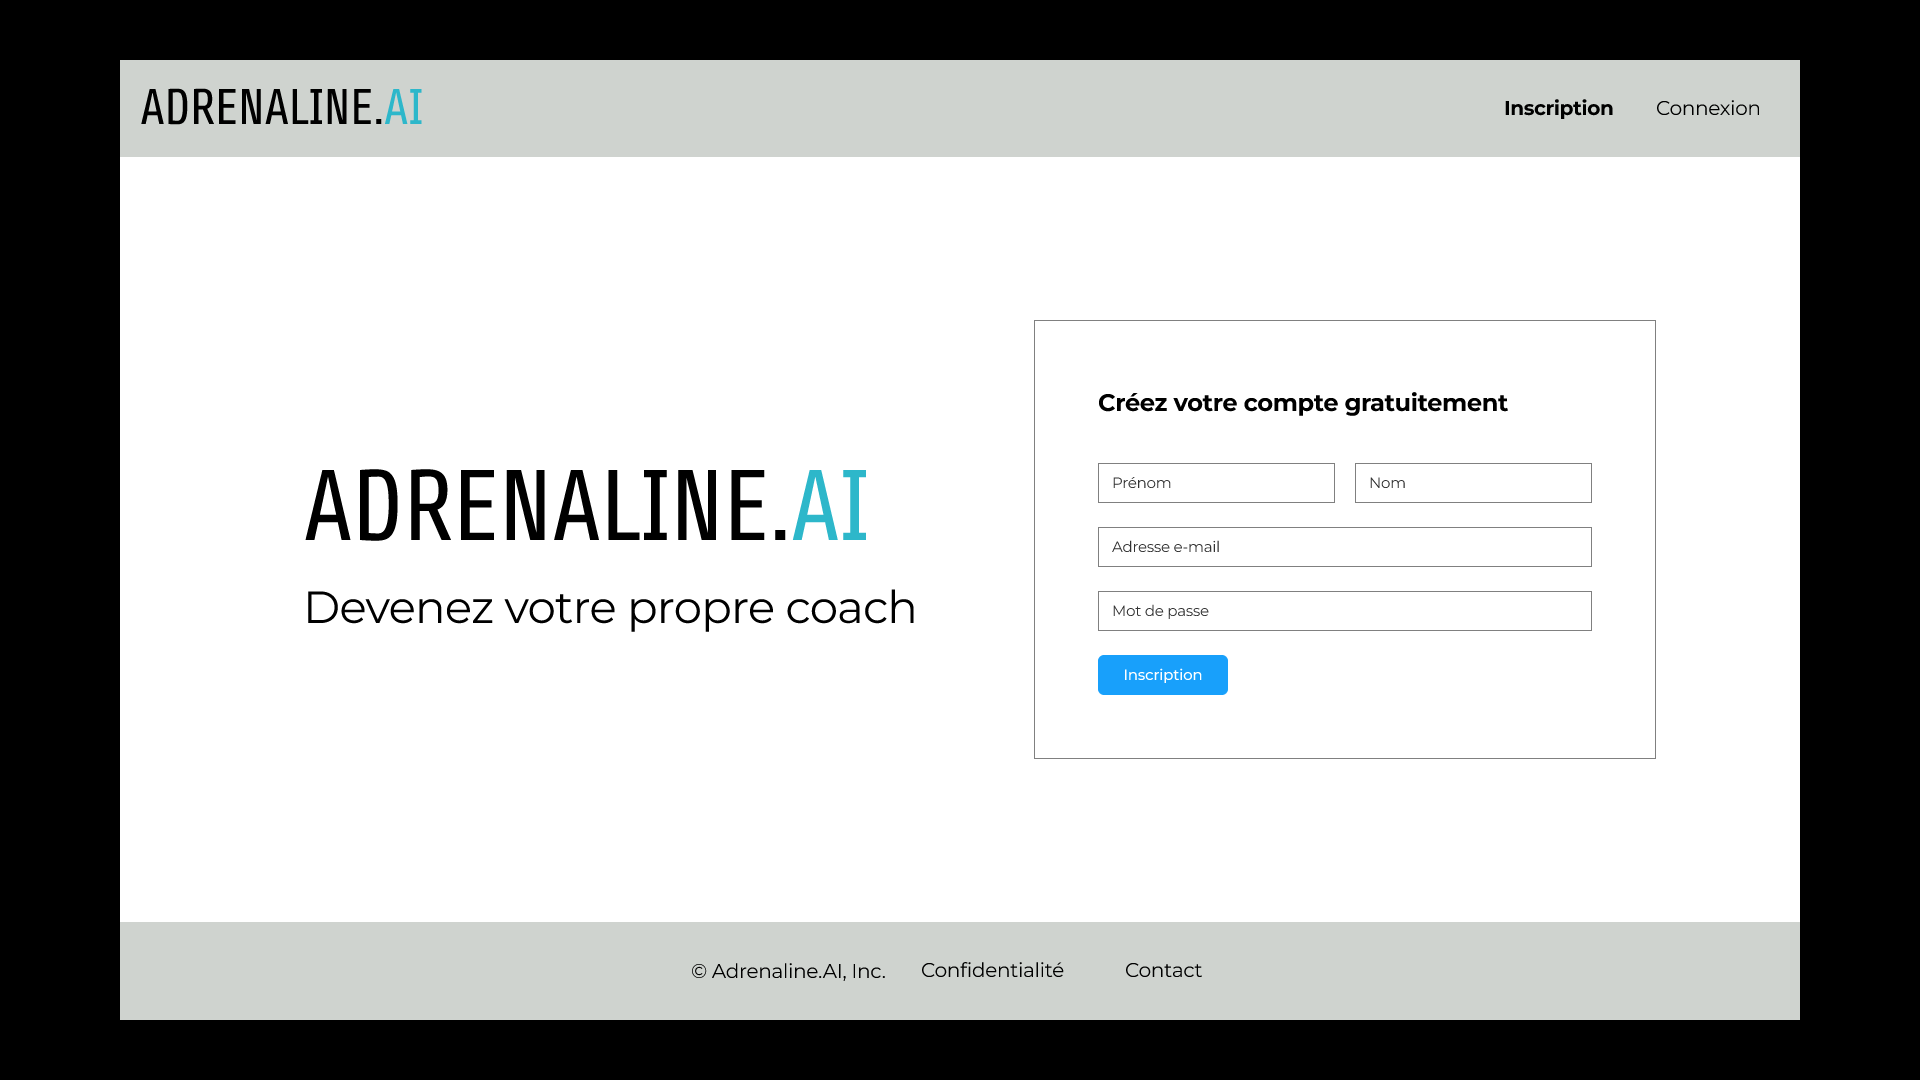
\includegraphics[width=12cm]{figma2}
        \centering
        \caption{La fonctionnalité de présentation du prototype de Figma permet de naviguer sur notre maquette comme sur une vraie application.}
        \centering
    \end{figure}

    \section{Implémentation des fonctionnalités}
    Cette partie traite de l'implémentation de l'application. Les fonctionnalités présentées dans le cahier des charges sont abordées individuellement.
    \subsection{Fonctionnalité 1 - recommandations d'entraînement}

    L'entraînement quotidien recommandé pour l'utilisateur est disponible sur la page web à l'URL /recommended\_workout. Lorsqu'une requête GET est envoyée à cette URL, plusieurs choses se passent :
    \begin{itemize}
        \item le script Python qui implémente le serveur regarde si la personne qui fait la requête est authentifiée. Si ce n'est pas le cas, elle est automatiquement redirigée vers la page de connexion (plus d'informations concernant les mécanismes d'authentification sont disponibles dans la présentation de la fonctionnalité 4)
        \item on récupère ensuite les données concernant l'utilisateur dans la base de données MySQL
        \item ces données sont envoyées au service d'intelligence artificielle via une API (\textbf{non implémentée dans le cadre de ce dossier})
        \item l'API retourne une description de l'entraînement à proposer à l'utilisateur. Cette description est affichée sur la page web renvoyée au navigateur qui a fait la requête.
    \end{itemize}
    \begin{figure}[h!]
        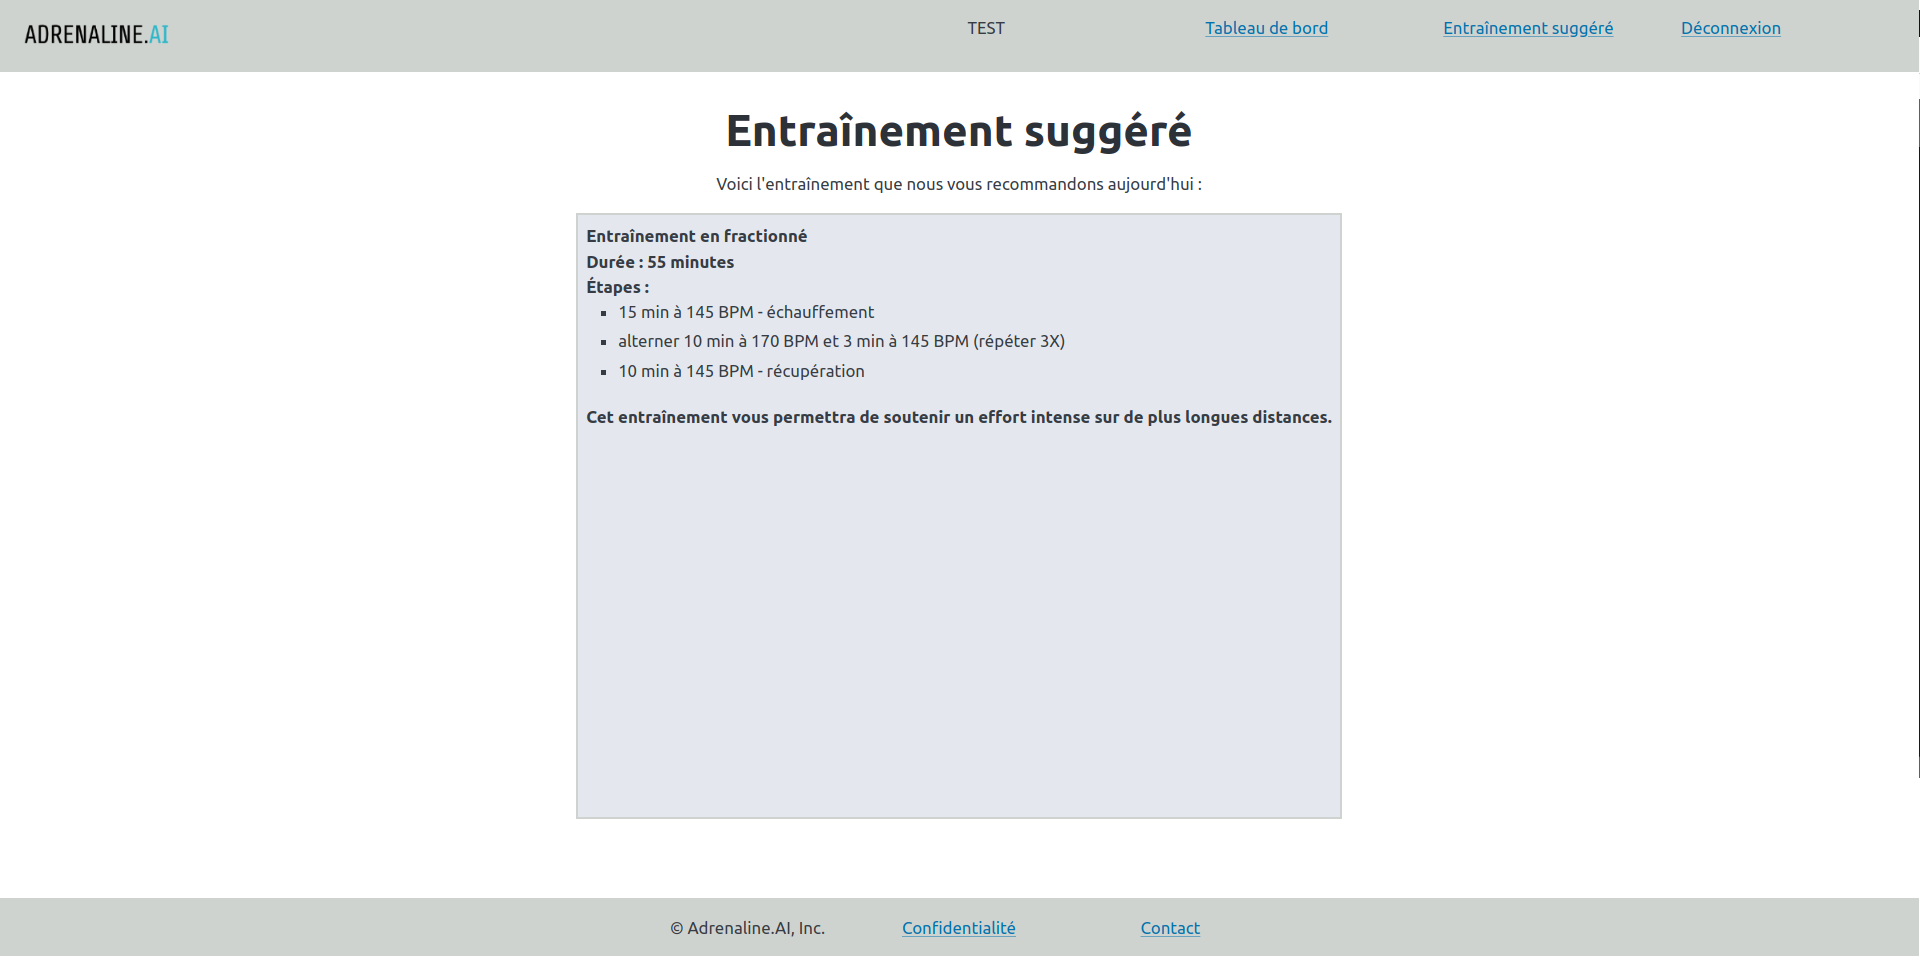
\includegraphics[width=12cm]{recommandation}
        \centering
        \caption{Affichage de l'entraînement recommandé dans l'application.}
        \centering
    \end{figure}

    \subsection{Fonctionnalité 2 - visualisation des données du coureur}

    Les utilisateurs peuvent visualiser les données les concernant sur la page /dashboard, qui est également la page d'accueil par défaut pour les utilisateurs authentifiés.
    \begin{figure}[h!]
        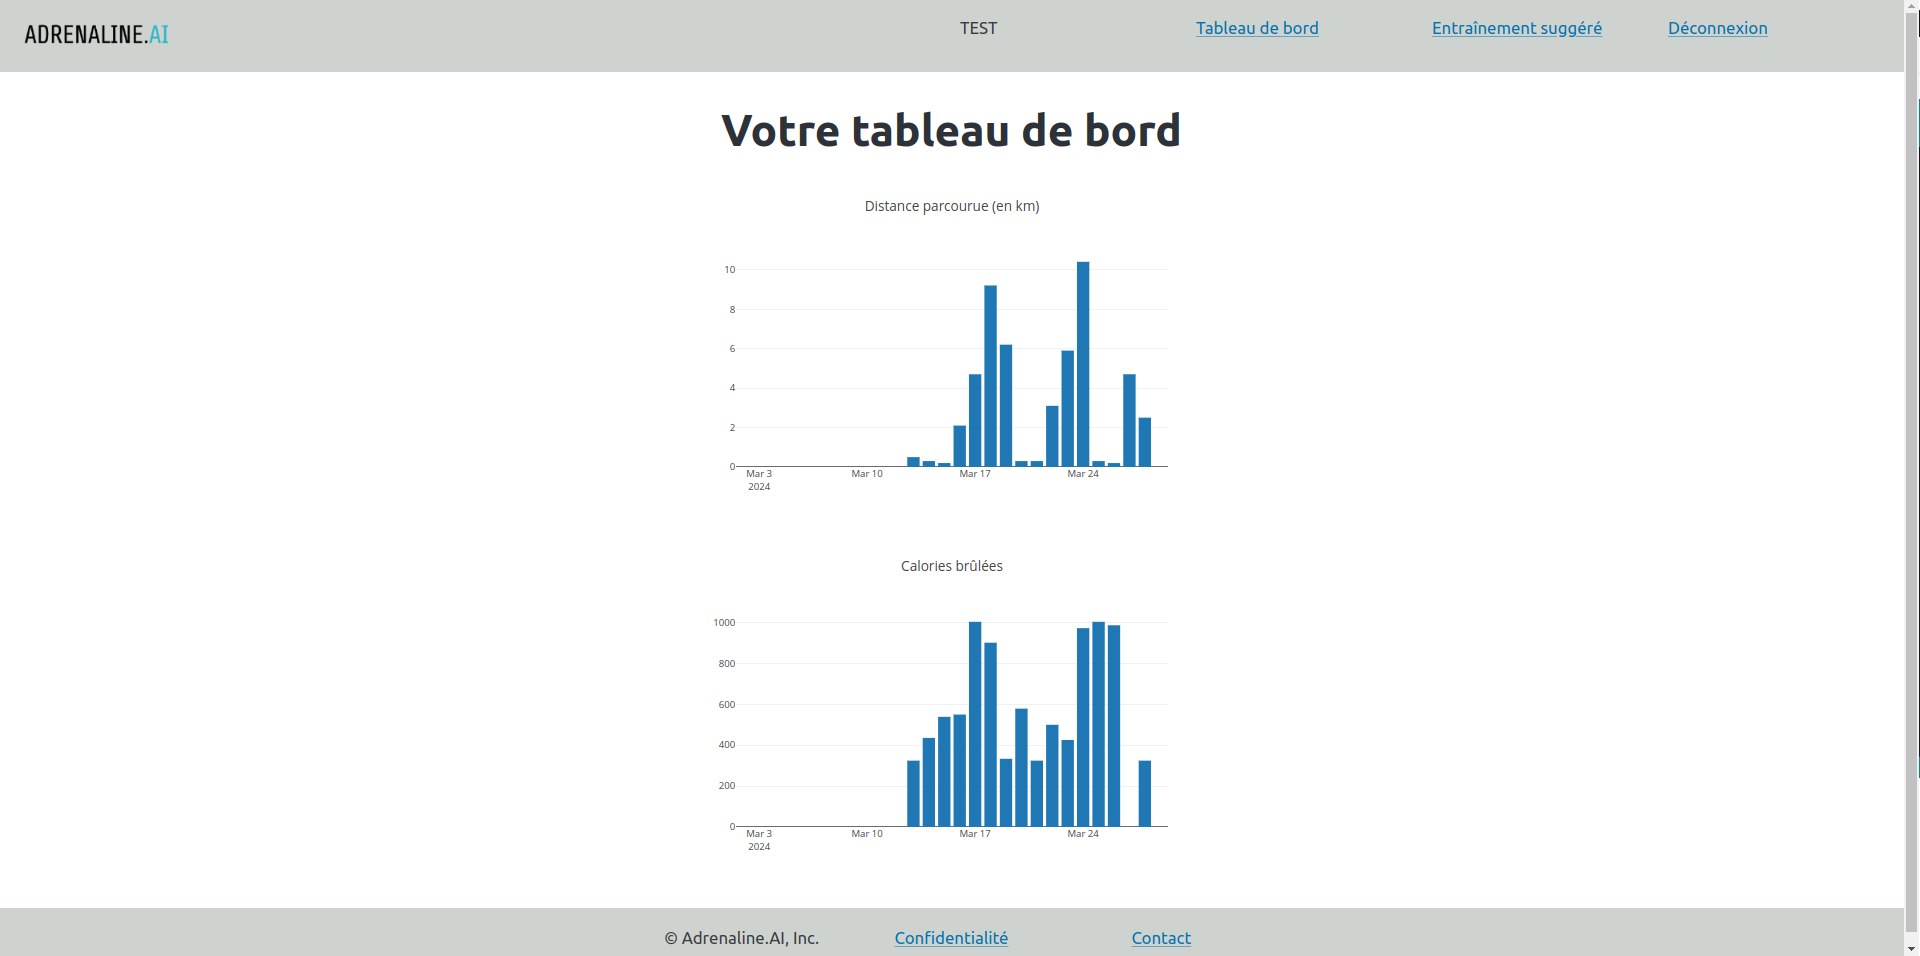
\includegraphics[width=12cm]{dashboard}
        \centering
        \caption{Affichage des données de l'utilisateur authentifié. L'affichage des graphiques est dynamique : l'utilisateur peut zoomer, dézoomer, télécharger le graphique en format PNG...}
        \centering
    \end{figure}

    Les graphiques en bâton présentés sur la page ont été générés avec la librairie \href{https://plotly.com/}{Plotly}. Plotly est conçu pour générer rapidement des graphiques dynamiques en JavaScript ou en Python (c'est la version JavaScript de la librairie qui est utilisée ici). 
    \subsection{Fonctionnalité 3 - gestion des données}
    Les données des utilisateurs sont stockées dans une base de données MySQL déployée sur Azure. En plus des mesures prises par la montre de l'utilisateur, la base de données contient toutes les informations relatives à l'authentification des utilisateurs (ce point sera abordé dans la section suivante).
    Cette base de données suit la structure présentée dans le MCD de la figure 6.

    \begin{figure}[h!]
        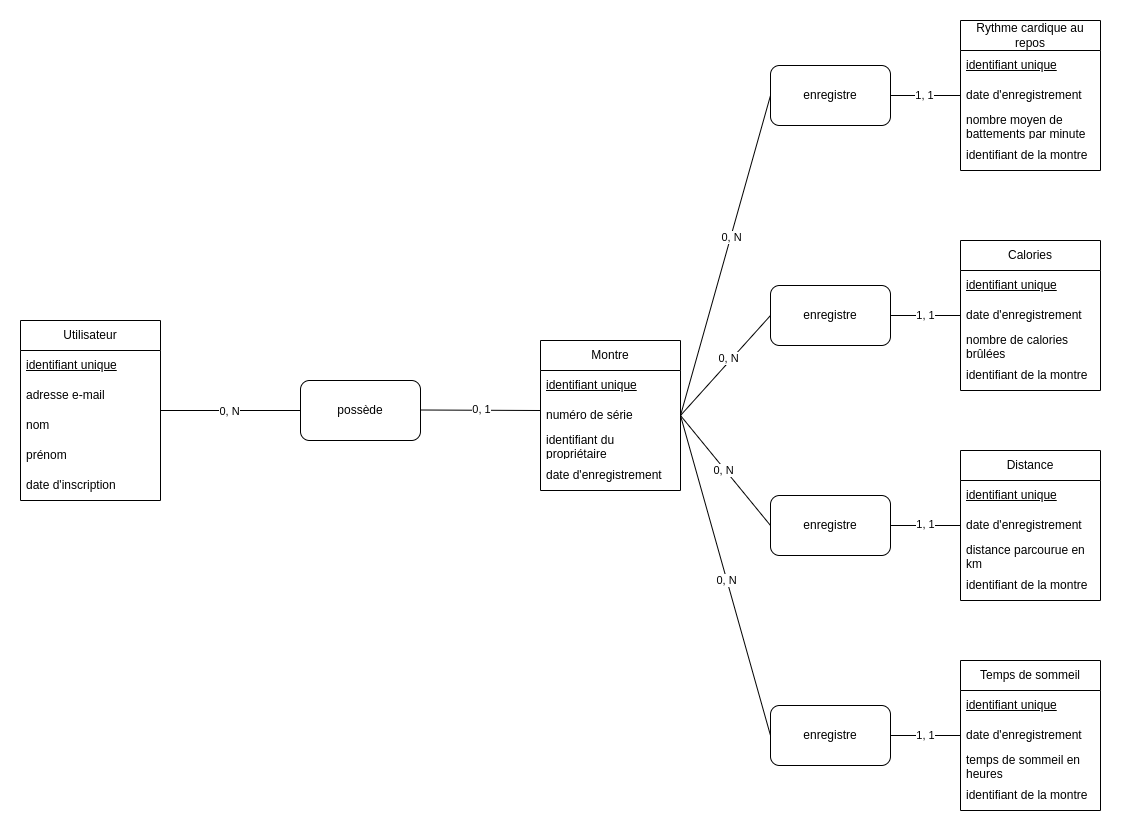
\includegraphics[width=12cm]{mcd_e4}
        \centering
        \caption{MCD (Modèle Conceptuel de Données) d'Adrenaline.AI.}
        \centering
    \end{figure}

    Ce MCD représente la logique de notre application. Les relations entre les différentes entités peuvent se résumer ainsi :
    \begin{itemize}
        \item un utilisateur peut possèder une ou plusieurs montres, ou aucune (il n'est pas nécessaire de posséder une montre pour créer un compte)
        \item une montre peut avoir un propriétaire, ou aucun (il est possible de posséder une montre sans avoir créé de compte)
        \item une montre est associée à un nombre arbitraire d'enregistrements de rythme cardiaque, calories, distance parcourue et temps de sommeil. En revanche, chaque enregistrement est associé à une et une seule montre.
    \end{itemize}

    Créer la base de données basée sur ce modèle conceptuel nous amène à la structure présentée dans la figure 7. En plus des éléments déjà présents dans le MCD, ce schéma introduit des éléments suivants dans la table 'users' : un hash de password et un 'salt' associé. Ces valeurs seront expliquées en détail dans la section suivante. 

    \begin{figure}[h!]
        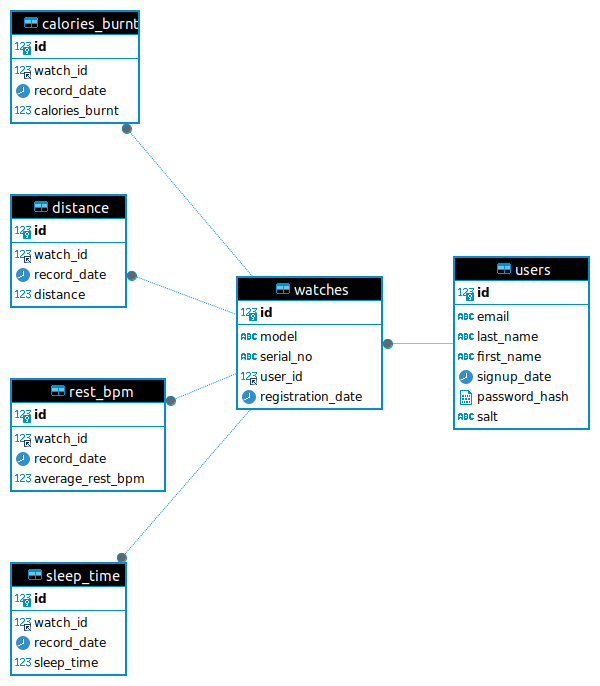
\includegraphics[width=12cm]{bdd}
        \centering
        \caption{Schéma de notre base de données généré par DBeaver.}
        \centering
    \end{figure}
    
    \subsection{Fonctionnalité 4 - gestion des utilisateurs}

    L'authentification des utilisateurs passe par la création d'un compte. La gestion des utilisateurs dans Adrenaline.AI est implémentée par plusieurs composants :
    \begin{itemize}
        \item le front-end, avec trois éléments d'interface :
        \begin{itemize}
            \item une page d'inscription à l'url /sign\_up, avec un formulaire pour créer un compte
            \item une page de connexion à l'url /sign\_in, avec un formulaire pour s'authentifier en entrant son adresse e-mail et son mot de passe.
            \item un lien pour se déconnecter et revenir à la page de connexion.
        \end{itemize}
        \item le back-end codé avec Flask, qui interroge la base de données pour traiter les demandes d'authentification et de création de compte. Il assure tous les contrôles nécessaires à la gestion des utilisateurs en vérifiant notamment qu'un utilisateur qui essaie de se connecter existe bien dans la base de données, ou encore que le mot de passe entré est valide. Une autre fonction importante du back-end est de conserver les \textbf{variables de session}. Stockées dans une structure semblable à un dictionnaire, les valeurs de session sont des variables associées à un utilisateur de l'application qui persistent d'une requête à une autre. C'est ce type de mécanisme qui explique que les sites web ne nous demandent pas de nous authentifier à nouveau à chaque fois que nous changeons de page : le serveur garde en mémoire notre navigateur. Dans Adrenaline.AI, nous stockons l'e-mail de l'utilisateur dans la variable 'username' lorsqu'il s'authentifie. Si cette variable n'existe pas, alors le serveur sait que l'utilisateur qui lui a envoyé une requête n'est pas authentifié.
        \item la base de données MySQL, que le serveur consulte pour assurer les tâches d'authentification.
    \end{itemize}

    La sécurité des données des utilisateurs est un aspect important du cahier des charges. Plusieurs mécanismes de sécurité sont mis en place pour empêcher des acteurs mal intentionnés de voler ou détruire des données.

    Le premier de ces mécanismes est le \textbf{hashing des mots de passe}. Plus tôt, nous avons affirmé que la table 'users' stocke les mots de passe des utilisateurs. En réalité ce n'est pas les mots de passe des utilisateurs qui sont stockés mais des \textbf{hashs} de ces mots de passe, autrement dit des empreintes cryptographiques.

    En cryptographie, une fonction de hashing (hachage en français) est une fonction mathématique qui associe à des valeurs de taille arbitraire des valeurs de taille fixe. Il en résulte un hash (ou \textbf{digest}), soit une séquence de bits souvent affichée en base hexadécimale pour plus de clarté. La figure 8 nous donne un exemple de fonction de hashing.

    L'une des utilisations du hashing est de sécuriser le stockage de mots de passe dans des bases de données. Ce processus fonctionne comme suit :
    \begin{itemize}
        \item lors de la création d'un utilisateur, on calcule le hash du mot de passe qu'il a entré et on le stocke dans la base de données
        \item quand un utilisateur veut s'authentifier, on calcule le hash du mot de passe qu'il a entré et on le compare à celui entré dans la base de données. Si les deux sont identiques, la connexion est autorisée.
    \end{itemize} 
    L'avantage de cette technique est que même si un attaquant parvient à trouver le hash d'un mot de passe, voire des mots de passe de tous les utilisateurs, il ne pourra pas exploiter ces informations. En effet, le hashing est un processus à sens unique : \textbf{il est (en théorie) impossible de trouver un mot de passe à partir de son hash}.
    \begin{figure}[h!]
        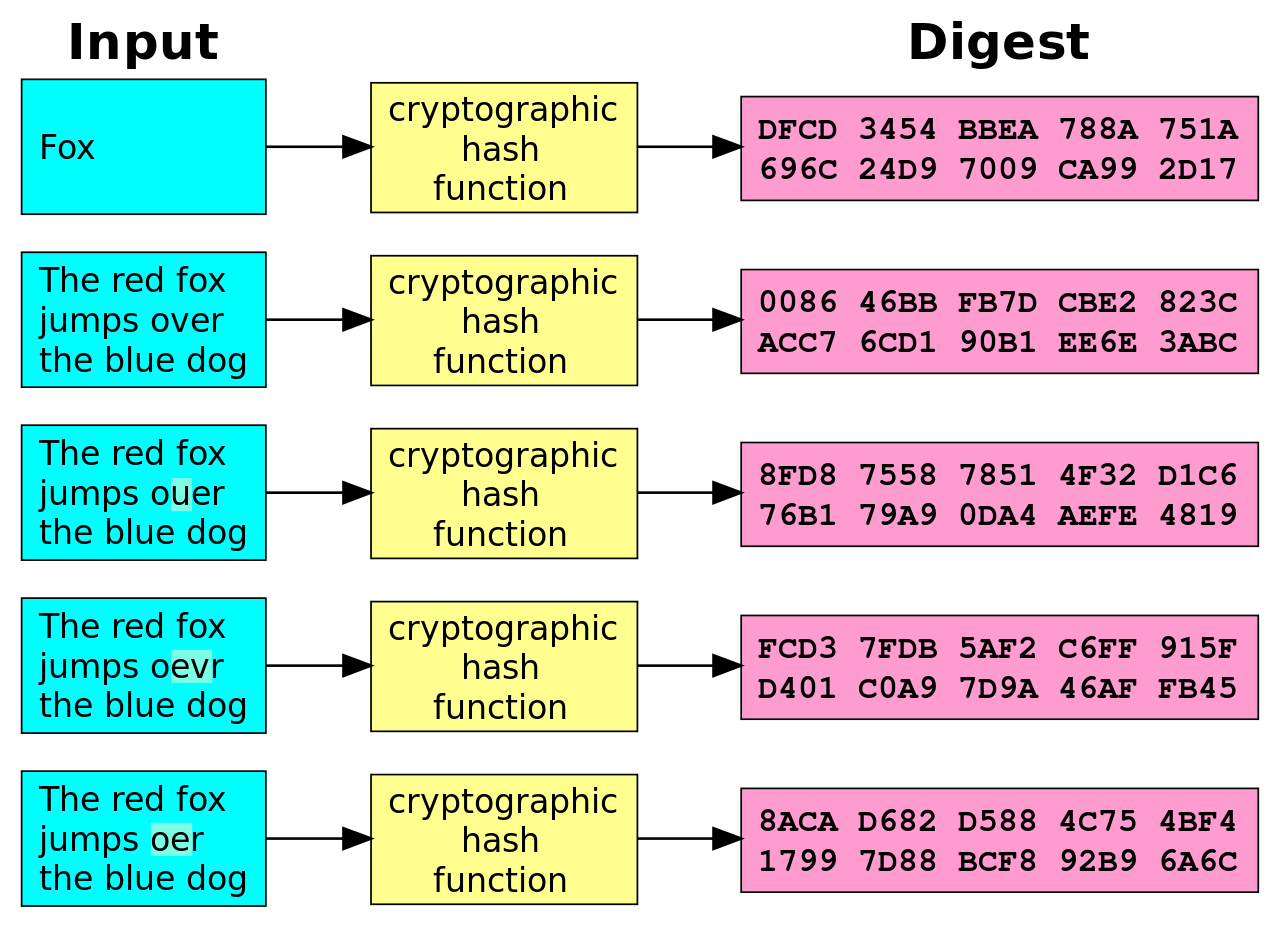
\includegraphics[width=12cm]{hashing}
        \centering
        \caption{Représentation d'une fonction de hashing. Les chaînes de caractères données à la fonction cryptographique, en bleu, sont converties en données binaires de longueur fixe.}
        \centering
    \end{figure}
    Pour renforcer la sécurité de l'authentification, une autre donnée a été ajoutée à la table 'users' : le \textbf{salt} ('sel' en français). Un salt est une séquence de bits aléatoire concaténée au mot de passe de l'utilisateur avant d'en calculer le hash. Cette technique sert à protéger notre système d'un type d'attaque qui utilise ce qu'on appelle des 'rainbow tables'. Les rainbow tables sont des tables qui stockent des paires prédéfinies de mots de passe et leur hash correspondant. Ajouter un salt aléatoire à nos mots de passe augmente considérablement la taille que devrait avoir cette table pour couvrir tous les mots de passe.
    
    En plus du hashing, d'autres mécanismes de sécurité ont été mis en place pour protéger les données des utilisateurs ou garantir le bon fonctionnement de l'application. Tout d'abord, les variables de configuration sensibles comme les identifiants de la base de données sont stockées dans des variables d'environnement, et pas dans le code. Par ailleurs, des mesures ont été prises pour empêcher les \textbf{injections SQL}. Une injection SQL est un type de cyberattaque qui consiste à exécuter du code SQL à l'insu des développeurs, par exemple en entrant du code dans un champ de formulaire. Voici un exemple de modification réalisée pour se protéger des injections  SQL dans le fichier utils.py :
    \begin{verbatim}
        # DANGEREUX
        query = f"""SELECT * FROM users WHERE email = {email}""" 
        c.execute(query)
        # PROTÉGÉ
        query = """SELECT * FROM users WHERE email = %s""" 
        query_vars = (email, )
        c.execute(query, query_vars)
    \end{verbatim}
    Dans l'exemple ci-dessus, l'utilisateur pourrait exploiter la première requête en entrant "email OR 1=1", par exemple. Comme la deuxième condition (1=1) est toujours vraie, cette requête renverrait la totalité de la table 'users', et pourrait donc potentiellement donner accès à des informations sensibles. Utiliser la deuxième méthode permet d'éviter ça.


    \section{Tests}

    La qualité du projet est assurée par des tests qui vérifient le bon fonctionnement du code. Ces tests visent principalement à garantir que l'application ne comporte pas de failles de sécurité et que les requêtes envoyées au serveur redirigent bien l'utilisateur vers les bonnes pages. Ces tests sont codés avec le framework de test \textbf{pytest}. Les tests sont implémentés dans le fichier \href{https://github.com/vinpap/adrenaline.ai/blob/main/test_app.py}{test\_app.py} et servent à vérifier le bon fonctionnement des différentes pages du site web. Voici une liste des tests réalisés :
    \begin{itemize}
        \item test\_index : vérifie que l'utilisateur est redirigé vers la bonne page selon qu'il est connecté ou non (/dashboard s'il est connecté, /sign\_in sinon)
        \item test\_sign\_in : vérifie que la page de connexion gère bien les différents scénarios (nom d'utilisateur et mot de passe valides, identifiants invalides, utilisateur qui entre du code SQL dans le champ du nom d'utilisateur...)
        \item test\_sign\_up : vérifie qu'il est bien impossible de recréer un compte déjà existant via le formulaire à l'adresse /sign\_up
        \item test\_logout : ce test s'assure qu'un utilisateur est bien déconnecté lorsqu'il envoit une requête à /logout
        \item test\_dasboard : vérifie qu'il est impossible de se connecter au tableau de bord sans être préalablement connecté
        \item test\_recommended\_workout : effectue la même vérification à l'adresse /recommended\_workout.
    \end{itemize}
    
    Voici un exemple de test unitaire avec test\_index :
    \begin{verbatim}
        def test_index(client):
            """
            Tests the root path by making sure it redirects to the 
            correct page (/dashboard if the user is signed in,
            /sign_in otherwise).
            """

            response = client.get("/", follow_redirects=True)
            assert response.request.path == "/sign_in"


            with client.session_transaction() as session:
                session["username"] = "TEST_USER"
            signed_in_response = client.get("/", follow_redirects=True)
            assert signed_in_response.request.path == "/dashboard"
    \end{verbatim}

    \section{Intégration et déploiement continus}

    Bien qu'il soit possible d'exécuter manuellement les tests ci-dessus, dans la pratique il est plus fiable d'automatiser leur exécution. Pour cela, nous utilisons \textbf{GitHub Action}, une fonctionnalité qui nous permet de réaliser des actions automatiquement lorsque des \textbf{déclencheurs} sont activés, autrement dit lorsque certains événements spécifiques surviennent.

    La configuration de GitHub Action est réalisée dans le fichier \href{https://github.com/vinpap/adrenaline.ai/blob/main/.github/workflows/main_vincent-adrenaline-ai.yml}{main\_vincent-adrenaline-ai.yaml}. Les déclencheurs sont spécifiés au début du fichier :

    \begin{verbatim}
    on:
        push:
            branches:
                - main
        pull_request:
            branches:
                - main
    \end{verbatim}

    On remarquera que le fichier liste trois "jobs" : "test", "build" et "deploy". Ceux-ci correspondent à une liste de tâches que GitHub Action exécute lorsque du code est poussé sur la branche main ou que du code est fusionné sur cette branche. 

    Le job "test" indique quelles instructions doivent être réalisées pour mettre en place l'environnement des tests et exécuter ces derniers :

    \begin{verbatim}
        # Install pytest
        - name: Install pytest and dependencies
          run: |
            python -m pip install --upgrade pip
            pip install pipenv
            pipenv install
  
          # Run the tests
        - name: Run tests
          run: |
            pipenv run pytest
          env: 
            MYSQL_HOST: ${{ secrets.MYSQL_HOST }}
            MYSQL_USER: ${{ secrets.MYSQL_USER }}
            MYSQL_PWD: ${{ secrets.MYSQL_PWD }}
            MYSQL_DB_NAME: ${{ secrets.MYSQL_DB_NAME }}
            FLASK_SESSION_KEY: ${{ secrets.FLASK_SESSION_KEY }}
    \end{verbatim}

    Ces lignes incluent l'installation des dépendances nécessaires pour que les tests s'exécutent ainsi que la définition des variables d'environnement nécessaires, notamment pour que l'application sache où se trouve la base de données et comment s'y connecter. On notera l'utilisation de secrets GitHub afin de ne pas exposer des informations sensibles telles que le mot de passe de notre base de données.

    Exactement de la même manière, GitHub Action nous permet d'automatiser le déploiement de notre application en s'interfaçant directement avec Azure. Ceci est réalisé dans les jobs "build" et "deploy".
    \begin{figure}[h!]
        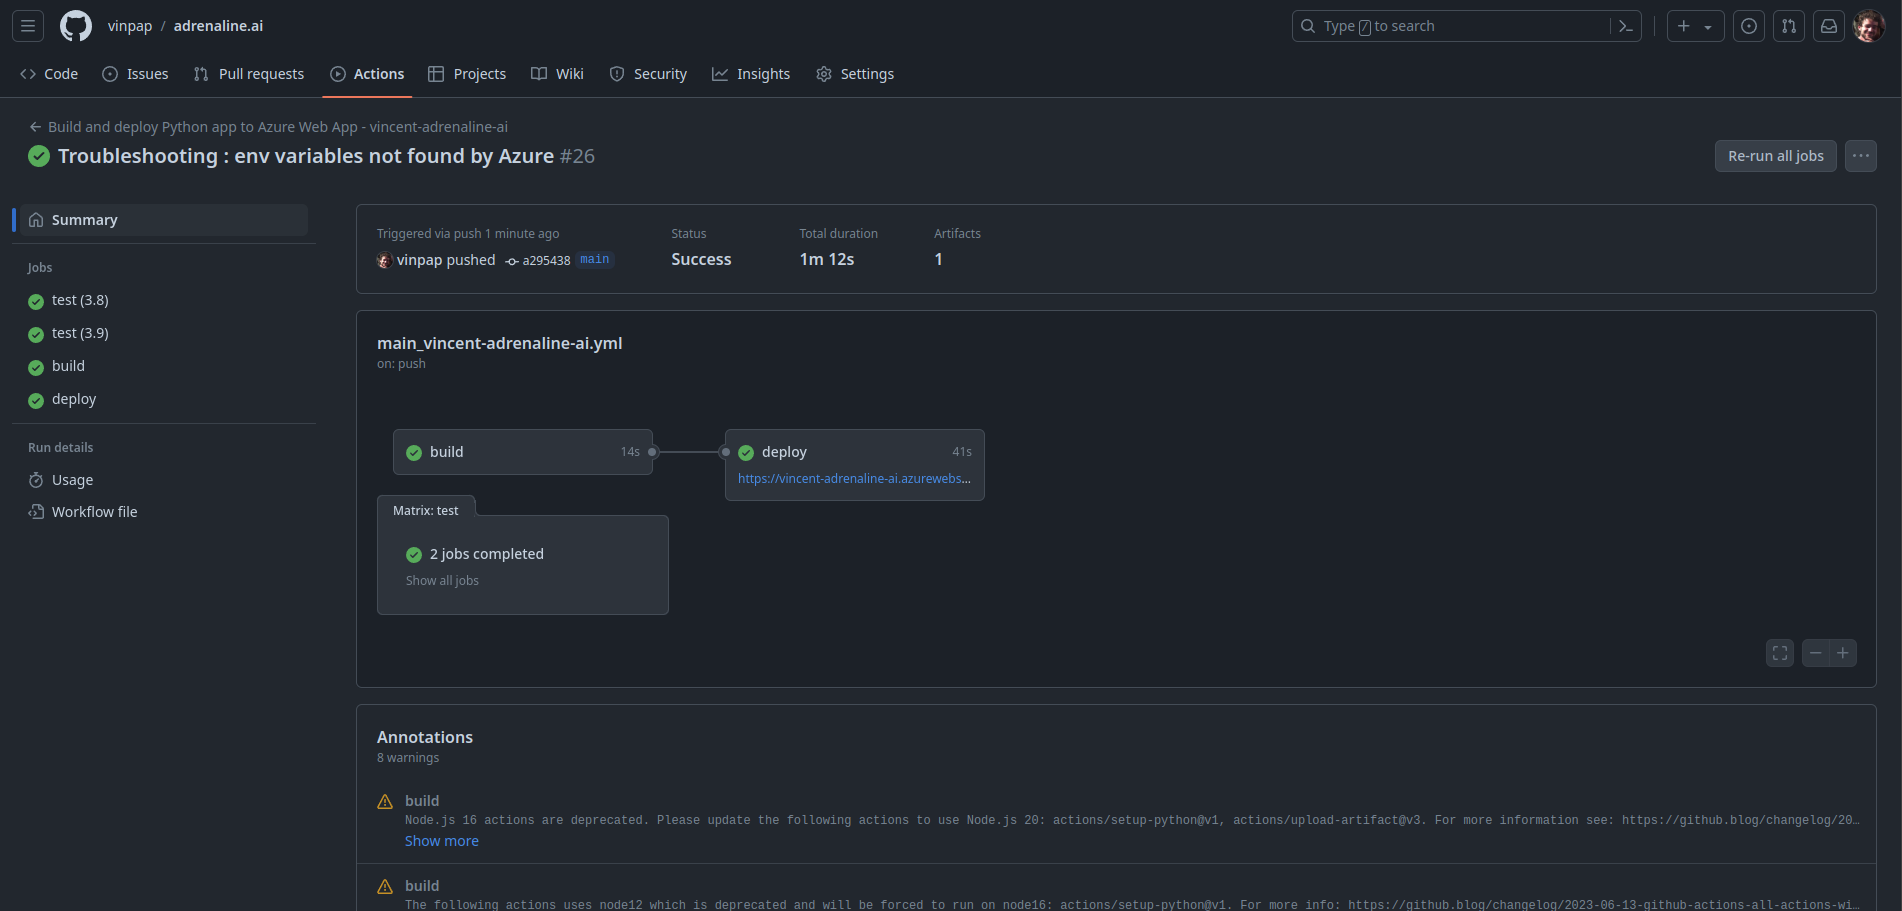
\includegraphics[width=12cm]{gh_action_1}
        \centering
        \caption{GitHub Action nous permet de visualiser l'exécution des tâches que nous avons paramétrées.}
        \centering
    \end{figure}
    
    Une version de l'application déployée sur Azure est disponible via \href{https://vincent-adrenaline-ai.azurewebsites.net/}{ce lien}. 

    \begin{figure}[h!]
        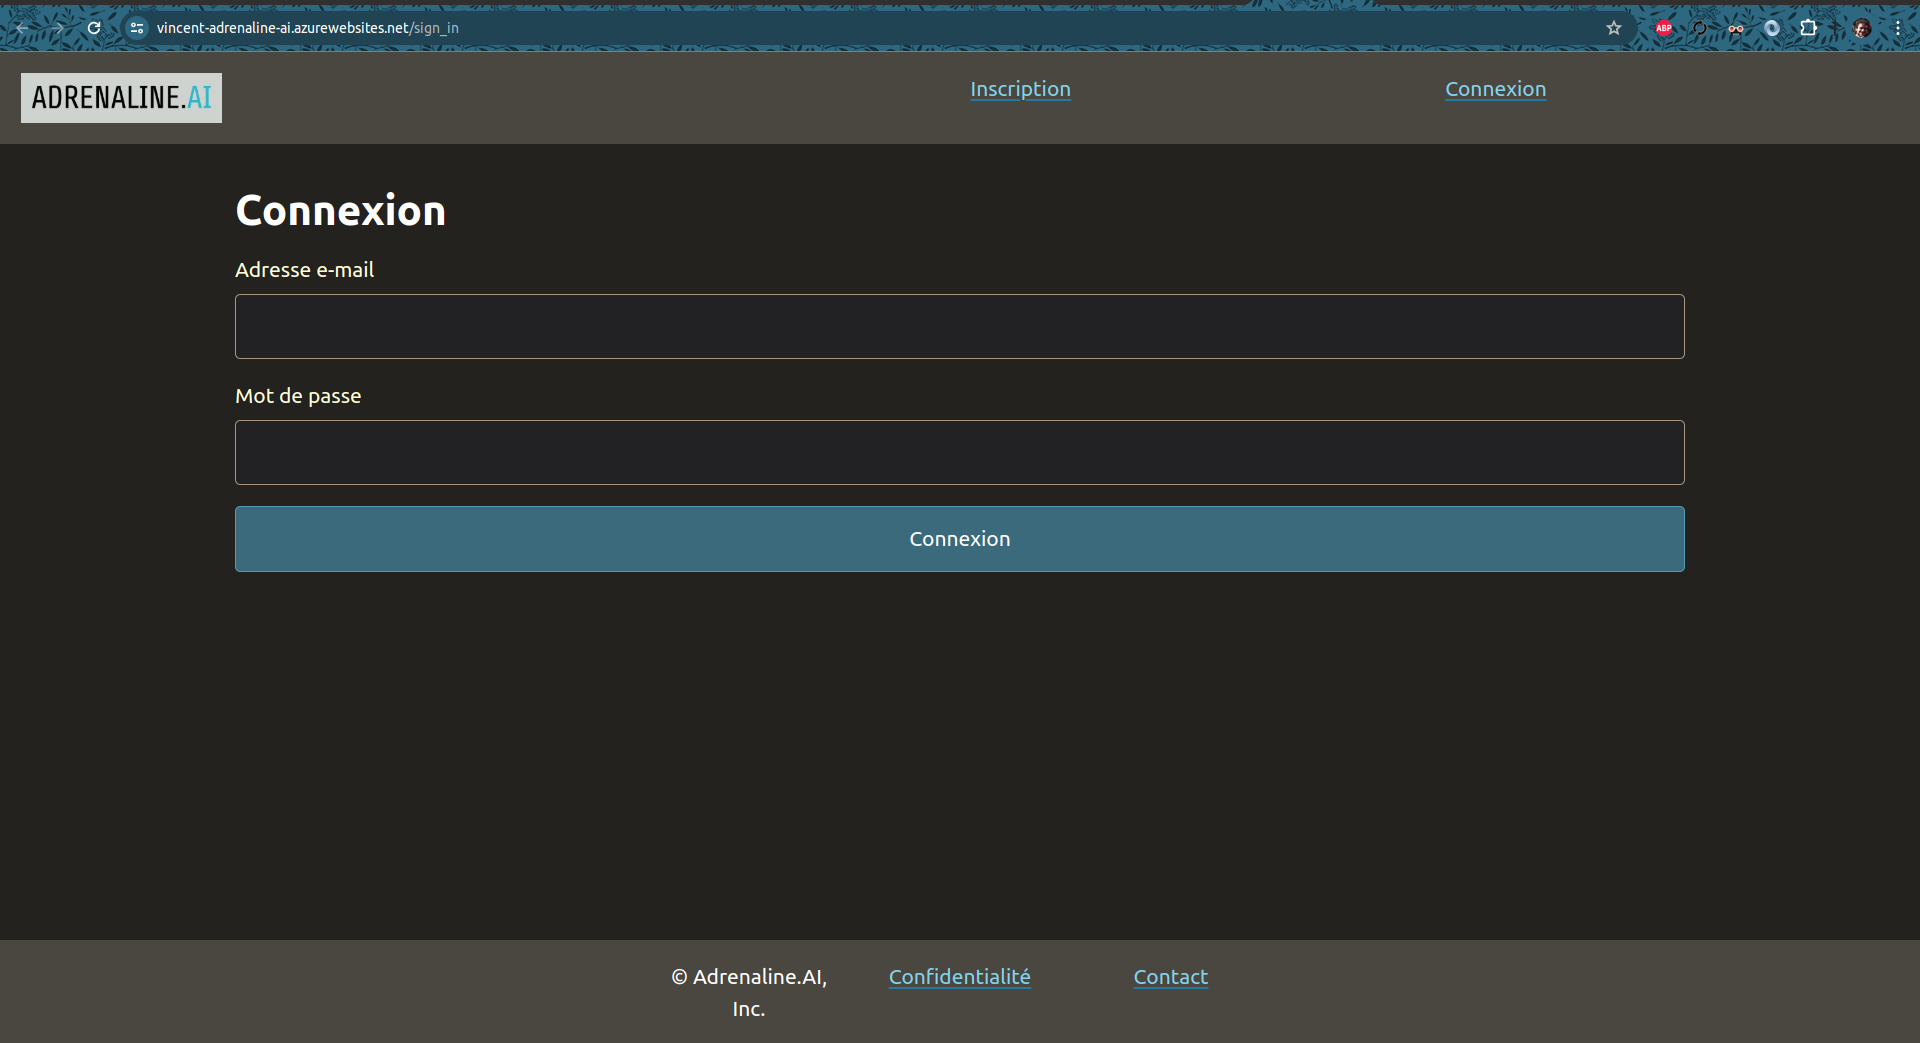
\includegraphics[width=12cm]{azure}
        \centering
        \caption{Une capture d'écran de notre application déployée sur Azure. Les variables d'environnement nécessaires à l'exécution ont été définies sur le portail de gestion d'Azure.}
        \centering
    \end{figure}
    
    \section{Documentation}
    \subsection{Déploiement}
    \subsection{Exécution des tests}
    \subsection{Développement et intégration continus}
    
    
    \newpage
    \section*{Conclusion}
    Résumer le travail accompli puis parler des difficultés potentielles et des axes d'amélioration
    
    

    \addcontentsline{toc}{section}{Conclusion}

    \end{document}